\documentclass[citeauthoryear]{llncs}
\usepackage{url}
\usepackage{cite}
\usepackage{listings}
\usepackage[utf8]{inputenc}
\usepackage{graphicx}
\usepackage{float}
\usepackage{verbatim}
\usepackage{eurosym}
\usepackage{haskell}


%\title{Assessing Modeling Languages, metrics and tools}
\title{Title}

%Exemplo para adição dos autores
\author{Pedro Faria \and Pedro Silva \and Ulisses Costa}

\institute{Department of Informatics, University of Minho}

\newcommand{\uml}{\textsf{UML}}
\newcommand{\xmi}{\textsf{XMI}}
\newcommand{\xml}{\textsf{XML}}
\newcommand{\entArch }{\textsf{Enterprise Architect}}
\newcommand{\sdmetrics}{\textsf{SDMetrics}}

\begin{document}
\maketitle

%%Abstract
\begin{abstract}
Any traditional engineering field has metrics to rigorously assess the quality of their products.
Engineers know that the output must satisfy the requirements, must comply with the production and market rules, and must be competitive.

Professionals in the new field of software engineering started a few years ago to define metrics to appraise their product: individual programs and software systems.
This concern motivates the need to assess not only the outcome but also the process and tools employed in its development.
In this context, assessing the quality of programming languages is a legitimate objective;
in a similar way, it makes sense to be concerned with models and modeling approaches, as more and more people start the software development process by a modeling phase.

In this paper we introduce and motivate the assessment of models quality in the Software Development cycle.
After the general discussion of this topic, we focus the attention on the most popular modeling language -- the UML -- presenting metrics.
Through a Case-Study, we present and explore two tools.
To conclude we identify what is still lacking in the tools side.

%In the paper we discuss the quality of modeling languages, introducing and motivating the topic, presenting metrics, and comparing tools.
\end{abstract}

\keywords Software Metrics, Haskell, Traversal Strategies, RoR, Perl

%%Introdução
\section{Introduction}
Quantitative measurements are essential in all sciences, and computer science is no exception.
Although Software Metrics aren't often used in Software Development, there has been an effort on the computer science community to develop and improve this metrics. 
The goal is to make them valuable in many aspects, such as quality assurance.\\
We present a static code analyser, that by measuring a set of metrics over C code, will give a notion of quality to the user. The software is able to generate
reports in \LaTeX~and in \textit{XML} format.\\
A system for managing programming contests, was chosen as the case study.
The competitors submit source code, which is their attempt to resolve a given problem.
The goal is not only to check if the solution is correct, but evaluate the quality of the submited code.\\
%We proceed to the next section, where we will show the system architecture, it's features and explain what is a programming contest, in this context.
%Ending with the explanation of how the parsing tree for the metrics calculation is constructed.
%We also explain the implementation of the case study, which is available in two differente plataforms.
%In the last section, we introduce the \textit{API} of the Metrics calculation, and a summarized explanation of each calculated metric.


\section{Architecture and features}
As said before, our tool is a system for managing programming contests. It can be accessed trough a Web Interface which is a \textit{RoR}\footnote{Ruby on Rails - \url{http://rubyonrails.org/}} application, and some of it's features can also be used from the terminal, taking advantage of a \textit{Perl} written script.
In Figure \ref{fig:arq}, we present a diagram that shows a simplified version of the system architecture.

\begin{figure}[htbp]
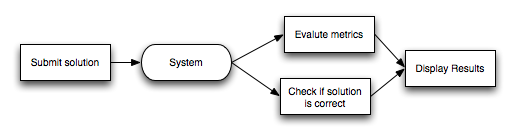
\includegraphics[scale=0.7]{images/arq}
\caption{Simplified System Architecture}
\label{fig:arq}
\end{figure}

\subsection{\textit{RoR} interface and \textit{Perl} interface}
As it would be expected, our system allows the creation of new contests, where among other things,
we can stipulate the date in which the contest starts and ends, and also it's durations.
Several exercises can be added to each contest, either manually, or by submitting one or more xml files.
An exercise has a description, a set of languages in which the competitors can solve the exercice, and a set of
input's and output's that the program will try to pass.
Having the contest propely created and being available to the competitors, they can register to be a contest participant,
and then start submitting their solutions to each of the contest exercises.  

\subsection{Parser and Traversal Strategies}
All of the work related to C files parsing, metrics extraction from them and output generation is done
using Haskell programming language. To extract some metrics we use a parser
library\footnote{Language.C - http://trac.sivity.net/language\_c/} done by Benedikt Huber under a GSoC (Google summer of code).
With this library we are able to construct a small parsing tree with the complete AST of C~\cite{Kernighan:1988:CPL:576122} and some GNU C extensions.\\
\indent To have an idea we only have 84 types of nodes (type constructors) in this tree, even so it is too big to traverse it by constructor, so
it was mandatory to use strategies to traverse this tree. We decide to use Strafusnki library~\cite{LV03-PADL}.


\newcommand{\metricsins}{\mathbin{>\mkern-7mu\circ\mkern-9mu>}}
\newcommand{\metricscat}{\mathbin{>\mkern-7mu+\mkern-11mu>}}

\section{Metrics and Assessment}\label{metrics}
To be able to manipulate and store the calculated metrics we have develop an API. Here are the relevent data types:
\begin{haskell*}
  \hskwd{data} Metrics
    & = & Metrics (Map MetricName MetricValue)\\
  \hskwd{type} MetricName
    & = & (Name,FileName,FunctionName)\\
  \hskwd{data} MetricValue
    & = & Num Double\\
    & | & Clone (Map FileDst [(Ocurrency, LineSrc, LineDst)])\\
    & | & Includes ([SystemIncludes],[Includes])
\end{haskell*}

We have used a Map to store our metrics, where the key is the triple $MetricName$. Some metrics just make sense when extracted regarding all the software package,
others may only be relevant regarding files and other may be extracted regarding a function. By letting some of empty fields in the triple we express this three categories
of metrics. Regarding the $MetricValue$ we can have multiple types of metrics, most of them just return a numerary value, the cosntructor $Num$. And then we have more specific
metrics related to clones found in the code, list of include and system includes.\\
\indent Now we present one of the most important function to append metrics. The power of \textit{Haskell} infix notation allow us to use comfortably this kind of functions.

\begin{haskell*}
  \metricsins ::  Metrics & \to& (MetricName, &MetricValue) \to Metrics\\
  m \metricsins (mn,mv) 
     &\mid &member mn m & = \hslet{fm  & = & fromMetrics m\\(Just mv') & = & lookup mn fm}
	{\hskwd{if} mv' \equiv mv \hskwd{then} m \hskwd{else} unpackPack ins m}\\
                            &\mid &otherwise   & = unpackPack ins m
	\hswhere{ins = insert mn mv}
\end{haskell*}

The previous function can be used when we want create a new metric, if so we must use $emptyMetrics$ as first paramenter.
The $unpackPack$ function used is a trick to remove the cosntructor, apply some function and return $Metrics$, could be defined as: $unpackPack~f \doteq toMetrics  \circ f \circ fromMetrics$.\\
\indent The following function can be used when the user already have some metrics calculated and want to concat them into one.

\begin{haskell*}
\metricscat & :: & Metrics \to Metrics \to Metrics\\
m1 \metricscat m2 & = & toMetrics (union (fromMetrics m1) (fromMetrics m2))
\end{haskell*}

As an example we can use this function to take a list of $Metrics$ and concat all of them into just one $Metrics$ value: $foldl~(\metricscat)~emptyMetrics$


\chapter{Conclusão e Trabalho Futuro}\label{chap con} 
Ao longo de toda primeira fase modelamos os vários aspectos do nosso sistema. Na segunda fase partimos para a implementação do
sistema e focamos também a nossa atenção na exploração de um frontend para a linguagem C.\\
\\
Toda a modelação do sistema realizada, foi importante, devido à visão mais alargada que nos deu do problema e da sua resolução.
A implementação correu de forma tranquila, onde apenas pequenos ajustes se realizaram, em relação ao pensado na fase anterior.
O trabalho relativo à importação de enunciados e tentativas em formato XML, que tinha ficado incompleto na fase I, e foi na fase II
completado.\\
O sistema está no fim desta fase apto a receber as soluções dos utilizadores, tratá-las, apresentar resultados e fazer detecção e clonning.\\
Na fase II foi também dado inicio ao desenvolvimento de uma interface em linha de comandos escrita em Perl, que alarga a acessibilidade à
aplicação, deixando do acesso à mesma estar dependente de um browser.\\
Ainda nesta fase a exploração do frontend \textit{Language.C} também deu os primeiros passos.\\
Neste momento da fase III esta ferramenta esta completamente dominada e partimos para a exploração de técnicas de programação genérica que
implemente estratégias de percorrer árvores de parsing, para conseguirmos extraír informação sobre o código que recebemos de input.
\\
Cremos que no fim desta fase III, o desenvolvimento da aplicação está terminado, foram corrigidos alguns bugs, a
interface está mais apelativa e intuitiva.\\

Para a próxima fase espera-nos o término da a aplicação pelo terminal e a aplicação de muito mais métricas e geração de um report com os resultados.

\section*{Acknowledgments}
The authors wish to thank Professor João Saraiva for the inpiration and for having guided this work.


%%Biblio
\bibliographystyle{alpha}
\bibliography{demoPaper}

\end{document} 
